\documentclass{standalone}
\usepackage{tikz}
\usepackage{ctex,siunitx}
\usepackage{tkz-euclide}
\usepackage{amsmath}
\usetikzlibrary{patterns, calc}
\usetikzlibrary {decorations.pathmorphing, decorations.pathreplacing, decorations.shapes,}
\begin{document}
\small
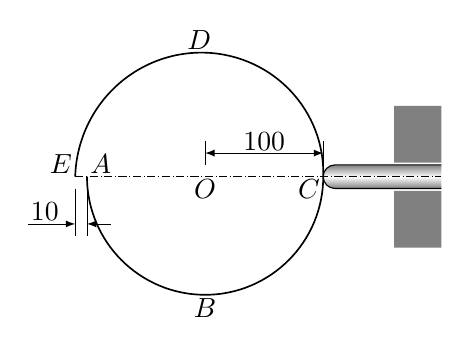
\begin{tikzpicture}[>=latex,scale=1.5,inner sep=1pt]
  \draw [semithick] (-1,0)arc(180:360:1);
  \draw [semithick,domain=0:180,samples=200] plot (\x:{1+\x/1800});
  \fill [gray](1.6,0.12)rectangle(2.0,0.6)(1.6,-0.12)rectangle(2.0,-0.6);
  \draw [top color=gray,bottom color=gray,middle color=white] (2,-0.1)--(1.1,-0.1)arc(270:90:0.1)--(2,0.1);
  \draw [very thin,densely dashdotted] (-1.1,0)--(2.0,0);
  \draw [very thin](-1.1,-.1)--(-1.1,-.5)(-1.0,-.1)--(-1.0,-.5);
  \draw [very thin](0,0.1)--(0,0.3)(1,0.1)--(1,0.3);
  \draw [very thin,<->](0,0.2)--(1,0.2)node[midway,above]{100};
  \draw [very thin,<-] (-1.0,-0.4)--(-0.8,-0.4);
  \draw [very thin,<-] (-1.1,-0.4)--(-1.5,-0.4)node[above right]{10};
  \node at (0,0) [below]{$O$};
  \node at (-1,0) [above right]{$A$};
  \node at (-0.05,1.05) [above]{$D$};
  \node at (0,-1) [below]{$B$};
  \node at (1,0) [below left]{$C$};
  \node at (-1.1,0) [above left]{$E$};
\end{tikzpicture}
\end{document}